%%%%%%%%%%%%%%%%%%%%%%%%%%%%%%%%%%%%%%%%%%%%%%%%%%%%%%%%%%%%%%%%%%%%%%%%%%%%%%%%
%
% Tab 1: Winner variants
%
%%%%%%%%%%%%%%%%%%%%%%%%%%%%%%%%%%%%%%%%%%%%%%%%%%%%%%%%%%%%%%%%%%%%%%%%%%%%%%%%

% full size table is table*
\begin{table*}[]
  \caption{Variants involved in 5 or more GWAS categories.}\label{tab:pleitropic_variants}
\centering
\scriptsize
\hline
\csvreader[separator=tab,
tabular=rrrrcp{0.6\textwidth},
head,
table head=\bfseries Chrom. & \bfseries Cytoband & \bfseries Pos. (hg38) & \bfseries Variant & \bfseries Cat. ct. & \bfseries GWAS Categories\\\hline,
]{fig/tab_rsid_most_pleiotropic.tsv}{}% use head of csv as column names
{\csvcoli\ & \csvcolii\ & \csvcoliii\ & \csvcoliv & \csvcolv & \csvcolvi}% specify your coloumns here
\hline
\end{table*}

%%%%%%%%%%%%%%%%%%%%%%%%%%%%%%%%%%%%%%%%%%%%%%%%%%%%%%%%%%%%%%%%%%%%%%%%%%%%%%%%
%
% Tab 2: Winner regions
%
%%%%%%%%%%%%%%%%%%%%%%%%%%%%%%%%%%%%%%%%%%%%%%%%%%%%%%%%%%%%%%%%%%%%%%%%%%%%%%%%

% full size table is table*
\begin{table*}[]
\caption{Pleiotropic regions involving 6 or more GWAS categories.}\label{tab:pleiotropic_regions}
\centering
\scriptsize
\hline
\csvreader[
separator=tab,
tabular=rrrrcp{0.5\textwidth},
head,
table head=\bfseries Chrom. & \bfseries Cytoband & \bfseries Start (hg38) & \bfseries End (hg38) & \bfseries Cat. ct. & \bfseries GWAS Categories\\\hline,
]{fig/tab_region_window_100000_pleio_highest.tsv}{}% use head of csv as column names
{\csvcoli\ & \csvcolii\ & \csvcoliii\ & \csvcoliv & \csvcolv & \csvcolvi}% specify your coloumns here
\hline
\end{table*}

%%%%%%%%%%%%%%%%%%%%%%%%%%%%%%%%%%%%%%%%%%%%%%%%%%%%%%%%%%%%%%%%%%%%%%%%%%%%%%%%
%
% Fig 5: Length histogram of regions
%
%%%%%%%%%%%%%%%%%%%%%%%%%%%%%%%%%%%%%%%%%%%%%%%%%%%%%%%%%%%%%%%%%%%%%%%%%%%%%%%%

\begin{figure*}[]
\centering
%
\includegraphics[width=0.33\textwidth]{\floatRelativePath/cmpt_pleiotropic_regions.py/regions_100000_length_hist.png}
%
\caption{\textbf{Length distribution of pleiotropic regions.} (\textbf{a}) TODO.} \label{fig:pleiotropy_region_distribution}
\end{figure*}

%%%%%%%%%%%%%%%%%%%%%%%%%%%%%%%%%%%%%%%%%%%%%%%%%%%%%%%%%%%%%%%%%%%%%%%%%%%%%%%%
%
% Fig 1: Histograms variants vs GWAS, egene and etissues
%
%%%%%%%%%%%%%%%%%%%%%%%%%%%%%%%%%%%%%%%%%%%%%%%%%%%%%%%%%%%%%%%%%%%%%%%%%%%%%%%%

\begin{figure*}[]
\centering
%
\begin{subfigure}[]{.32\textwidth}
\textbf{a}
\\
\includegraphics[width=\textwidth]{\floatRelativePath/plthst_gwas_egene_etissue.py/hist_gwas.png}
\end{subfigure}
%
\begin{subfigure}[]{.32\textwidth}
\textbf{b}
\\
\includegraphics[width=\textwidth]{\floatRelativePath/plthst_gwas_egene_etissue.py/hist_egene.png}
\end{subfigure}
%
\begin{subfigure}[]{.32\textwidth}
\textbf{c}
\\
\includegraphics[width=\textwidth]{\floatRelativePath/plthst_gwas_egene_etissue.py/hist_etissue.png}
\end{subfigure}
%
\caption{\textbf{Probability density of GWAS phenotypes, eGene or eQTL samples.} (\textbf{a}) TODO.} \label{fig:hist_gwas_egene_etissue}
\end{figure*}

%%%%%%%%%%%%%%%%%%%%%%%%%%%%%%%%%%%%%%%%%%%%%%%%%%%%%%%%%%%%%%%%%%%%%%%%%%%%%%%%
%
% Fig 2: Scatter plots of winner regions
%
%%%%%%%%%%%%%%%%%%%%%%%%%%%%%%%%%%%%%%%%%%%%%%%%%%%%%%%%%%%%%%%%%%%%%%%%%%%%%%%%


\begin{figure*}[!ht]

\begin{subfigure}[]{.33\textwidth}
\textbf{a}
\\
\includegraphics[width=\textwidth]{\floatRelativePath/pltsctr_x_per_rsid_y_gwas.py/count_per_rsid_chr5_start132239645_end132497907_categories8.png}
\end{subfigure}
%
\begin{subfigure}[]{.33\textwidth}
\textbf{b}
\\
\includegraphics[width=\textwidth]{\floatRelativePath/pltsctr_x_per_rsid_y_gwas.py/count_per_rsid_chr6_start31034839_end32478149_categories8.png}
\end{subfigure}
%
\begin{subfigure}[]{.33\textwidth}
\textbf{c}
\\
\includegraphics[width=\textwidth]{\floatRelativePath/pltsctr_x_per_rsid_y_gwas.py/count_per_rsid_chr12_start111395984_end111645358_categories11.png}
\end{subfigure}


\begin{subfigure}[]{.33\textwidth}
\textbf{d}
\\
\includegraphics[width=\textwidth]{\floatRelativePath/pltsctr_x_per_rsid_y_egene.py/count_per_rsid_chr5_start132239645_end132497907_categories8.png}
\end{subfigure}
%
\begin{subfigure}[]{.33\textwidth}
\textbf{e}
\\
\includegraphics[width=\textwidth]{\floatRelativePath/pltsctr_x_per_rsid_y_egene.py/count_per_rsid_chr6_start31034839_end32478149_categories8.png}
\end{subfigure}
%
\begin{subfigure}[]{.33\textwidth}
\textbf{f}
\\
\includegraphics[width=\textwidth]{\floatRelativePath/pltsctr_x_per_rsid_y_egene.py/count_per_rsid_chr12_start111395984_end111645358_categories11.png}
\end{subfigure}

\begin{subfigure}[]{.33\textwidth}
\textbf{g}
\\
\includegraphics[width=\textwidth]{\floatRelativePath/pltsctr_x_per_rsid_y_etissue.py/count_per_rsid_chr5_start132239645_end132497907_categories8.png}
\end{subfigure}
%
\begin{subfigure}[]{.33\textwidth}
\textbf{h}
\\
\includegraphics[width=\textwidth]{\floatRelativePath/pltsctr_x_per_rsid_y_etissue.py/count_per_rsid_chr6_start31034839_end32478149_categories8.png}
\end{subfigure}
%
\begin{subfigure}[]{.33\textwidth}
\textbf{i}
\\
\includegraphics[width=\textwidth]{\floatRelativePath/pltsctr_x_per_rsid_y_etissue.py/count_per_rsid_chr12_start111395984_end111645358_categories11.png}
\end{subfigure}

\caption{\textbf{Count of GWAS categories, eGenes and eTissues in pleiotropic genomic regions.} (\textbf{a,d,g}) Region 5:132,239,645-132,497,907, \textbf{b,e,h}) region 6:31,034,839-32,478,149,  and \textbf{c,g,i}) region 12:111,395,984-111,645,358} \label{fig:region_gwas_egenes_tissues}
%
\end{figure*}

%%%%%%%%%%%%%%%%%%%%%%%%%%%%%%%%%%%%%%%%%%%%%%%%%%%%%%%%%%%%%%%%%%%%%%%%%%%%%%%%
%
% Fig 3: VEP consequences
%
%%%%%%%%%%%%%%%%%%%%%%%%%%%%%%%%%%%%%%%%%%%%%%%%%%%%%%%%%%%%%%%%%%%%%%%%%%%%%%%%

\begin{figure*}[!]
\centering
%
\begin{subfigure}[]{.33\textwidth}
\textbf{a}
\\
\includegraphics[width=\textwidth]{\floatRelativePath/plt_vep_consequence.py/missense_variant.png}
%
\end{subfigure}
%
\begin{subfigure}[]{.33\textwidth}
\textbf{b}
\\
\includegraphics[width=\textwidth]{\floatRelativePath/plt_vep_consequence.py/splice_region_variant.png}
%
\end{subfigure}
%
\begin{subfigure}[]{.33\textwidth}
\textbf{c}
\\
\includegraphics[width=\textwidth]{\floatRelativePath/plt_vep_consequence.py/3_prime_UTR_variant.png}
%
\end{subfigure}
%
\caption{\textbf{Location of of variants computed as VEP consequence.} (\textbf{a}) TODO.} \label{fig:vep_consequence}
%
\end{figure*}

%%%%%%%%%%%%%%%%%%%%%%%%%%%%%%%%%%%%%%%%%%%%%%%%%%%%%%%%%%%%%%%%%%%%%%%%%%%%%%%%
%
% Fig 4: Violin plots. eGenes, etissues and gwas per variants
%
%%%%%%%%%%%%%%%%%%%%%%%%%%%%%%%%%%%%%%%%%%%%%%%%%%%%%%%%%%%%%%%%%%%%%%%%%%%%%%%%

\begin{figure*}[!]
\centering
%
\begin{subfigure}[]{.33\textwidth}
\textbf{a}
\\
\includegraphics[width=\textwidth]{\floatRelativePath/pltbox_x_per_variant_y_egene.py/plt.png}
\end{subfigure}
%
\begin{subfigure}[]{.33\textwidth}
\textbf{b}
\\
\includegraphics[width=\textwidth]{\floatRelativePath/pltbox_x_per_variant_egene_y_etissue.py/plt.png}
\end{subfigure}
%
\begin{subfigure}[]{.33\textwidth}
\textbf{c}
\\
\includegraphics[width=\textwidth]{\floatRelativePath/pltbox_x_per_variant_egene_etissue_y_gwas.py/plt.png}
\end{subfigure}
%
\caption{\textbf{Frequency of eGenes per variant, eTissues per variant-eGene and phenotypes per variant-eGene-eTissue.} (\textbf{a}) TODO.} \label{fig:freq_gwas_egene_etisue_per_variant}
%
\end{figure*}

%%%%%%%%%%%%%%%%%%%%%%%%%%%%%%%%%%%%%%%%%%%%%%%%%%%%%%%%%%%%%%%%%%%%%%%%%%%%%%%%
%
% Fig 6: TF count per GWAS category count
%
%%%%%%%%%%%%%%%%%%%%%%%%%%%%%%%%%%%%%%%%%%%%%%%%%%%%%%%%%%%%%%%%%%%%%%%%%%%%%%%%

\begin{figure*}[!]
\centering
%
\begin{subfigure}[]{.33\textwidth}
%
\includegraphics[width=\textwidth]{\floatRelativePath/pltbox_x_per_rsid_y_remaptf.py/bxplt_remaptf_per_rsid_flank_0.png}
\end{subfigure}
%
\caption{\textbf{Binding of transcription factors in the region (100 kb) around pleiotropic variants.} (\textbf{a}) TODO.} \label{fig:freq_tf_per_variant}
%
\end{figure*}

%%%%%%%%%%%%%%%%%%%%%%%%%%%%%%%%%%%%%%%%%%%%%%%%%%%%%%%%%%%%%%%%%%%%%%%%%%%%%%%%
%
% Fig 7: beta and log pval
%
%%%%%%%%%%%%%%%%%%%%%%%%%%%%%%%%%%%%%%%%%%%%%%%%%%%%%%%%%%%%%%%%%%%%%%%%%%%%%%%%

\begin{figure*}[!]
\centering
%
\begin{subfigure}[]{.33\textwidth}
\textbf{a}
\\
\includegraphics[width=\textwidth]{\floatRelativePath/pltbox_x_per_gwas_cat_y_beta.py/eqtl_beta.png}
\end{subfigure}
%
\begin{subfigure}[]{.33\textwidth}
\textbf{b}
\\
\includegraphics[width=\textwidth]{\floatRelativePath/pltbox_x_per_gwas_cat_y_beta.py/gwas_beta.png}
\end{subfigure}

\begin{subfigure}[]{.33\textwidth}
\textbf{c}
\\
\includegraphics[width=\textwidth]{\floatRelativePath/pltbox_x_per_gwas_cat_y_logpval.py/eqtl.png}
\end{subfigure}
%
\begin{subfigure}[]{.33\textwidth}
\textbf{d}
\\
\includegraphics[width=\textwidth]{\floatRelativePath/pltbox_x_per_gwas_cat_y_logpval.py/gwas.png}
\end{subfigure}

\caption{\textbf{TODO.} (\textbf{a}) TODO.} \label{fig:beta}
%
\end{figure*}

%%%%%%%%%%%%%%%%%%%%%%%%%%%%%%%%%%%%%%%%%%%%%%%%%%%%%%%%%%%%%%%%%%%%%%%%%%%%%%%%
%
% Fig 7: graphical conclusions
%
%%%%%%%%%%%%%%%%%%%%%%%%%%%%%%%%%%%%%%%%%%%%%%%%%%%%%%%%%%%%%%%%%%%%%%%%%%%%%%%%

\begin{figure*}[!]
\centering
%
\begin{subfigure}[]{\textwidth}

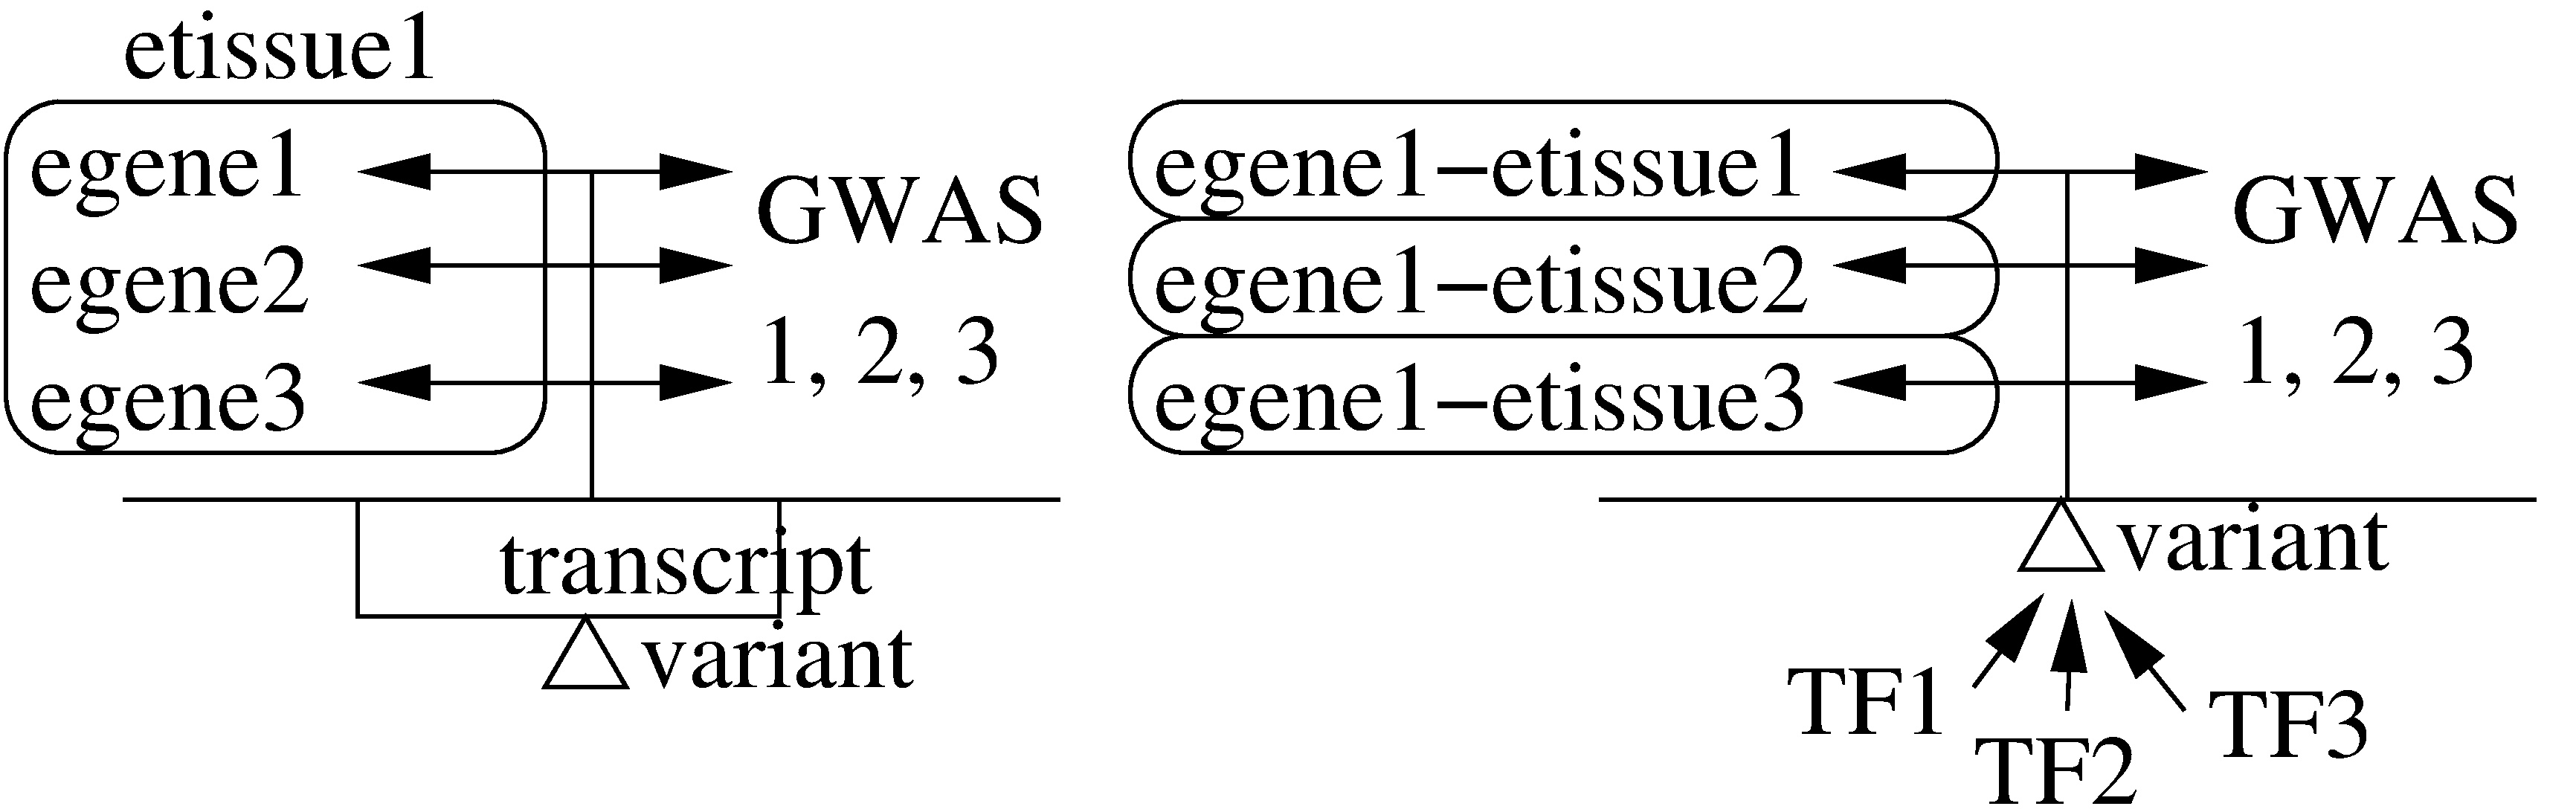
\includegraphics[width=\textwidth]{fig/graphical_summary.png}
\end{subfigure}

\caption{\textbf{Molecular mechanism of pleiotropy.} (We have observed three possible mechanisms resulting in pleiotropy. (Left) Pleiotropic variants have more eGenes. One explanation is that these variants are present in splicing regions. (Center) eGenes of pleiotropic variants are active in more eTissues, which might be explained from variants being bound by more transcription factors. (Right) eGenes/eTissues are associated with more GWAS phenotypes. This might be explained because the variants have more frequently a missense consequence.} \label{fig:beta}
%
\end{figure*}
